\subsubsection{Work Planning, Attendance and Actual Work}
\label{sec:conceptual-workforce}
The model separates expectations, daily presence and actual campaign participation.
WorkPlan groups one campaign's assignments for a working date. PlannedAssignment
identifies a worker and area, with optional PlannedWorkPeriod and PlannedBreak
records. These tables retain the proposal independently of subsequent actual work.
Figures~\ref{fig:er-planning} and~\ref{fig:er-actual-work} show planning and actual work,
respectively.

\begin{figure}[!htbp]
    \centering
    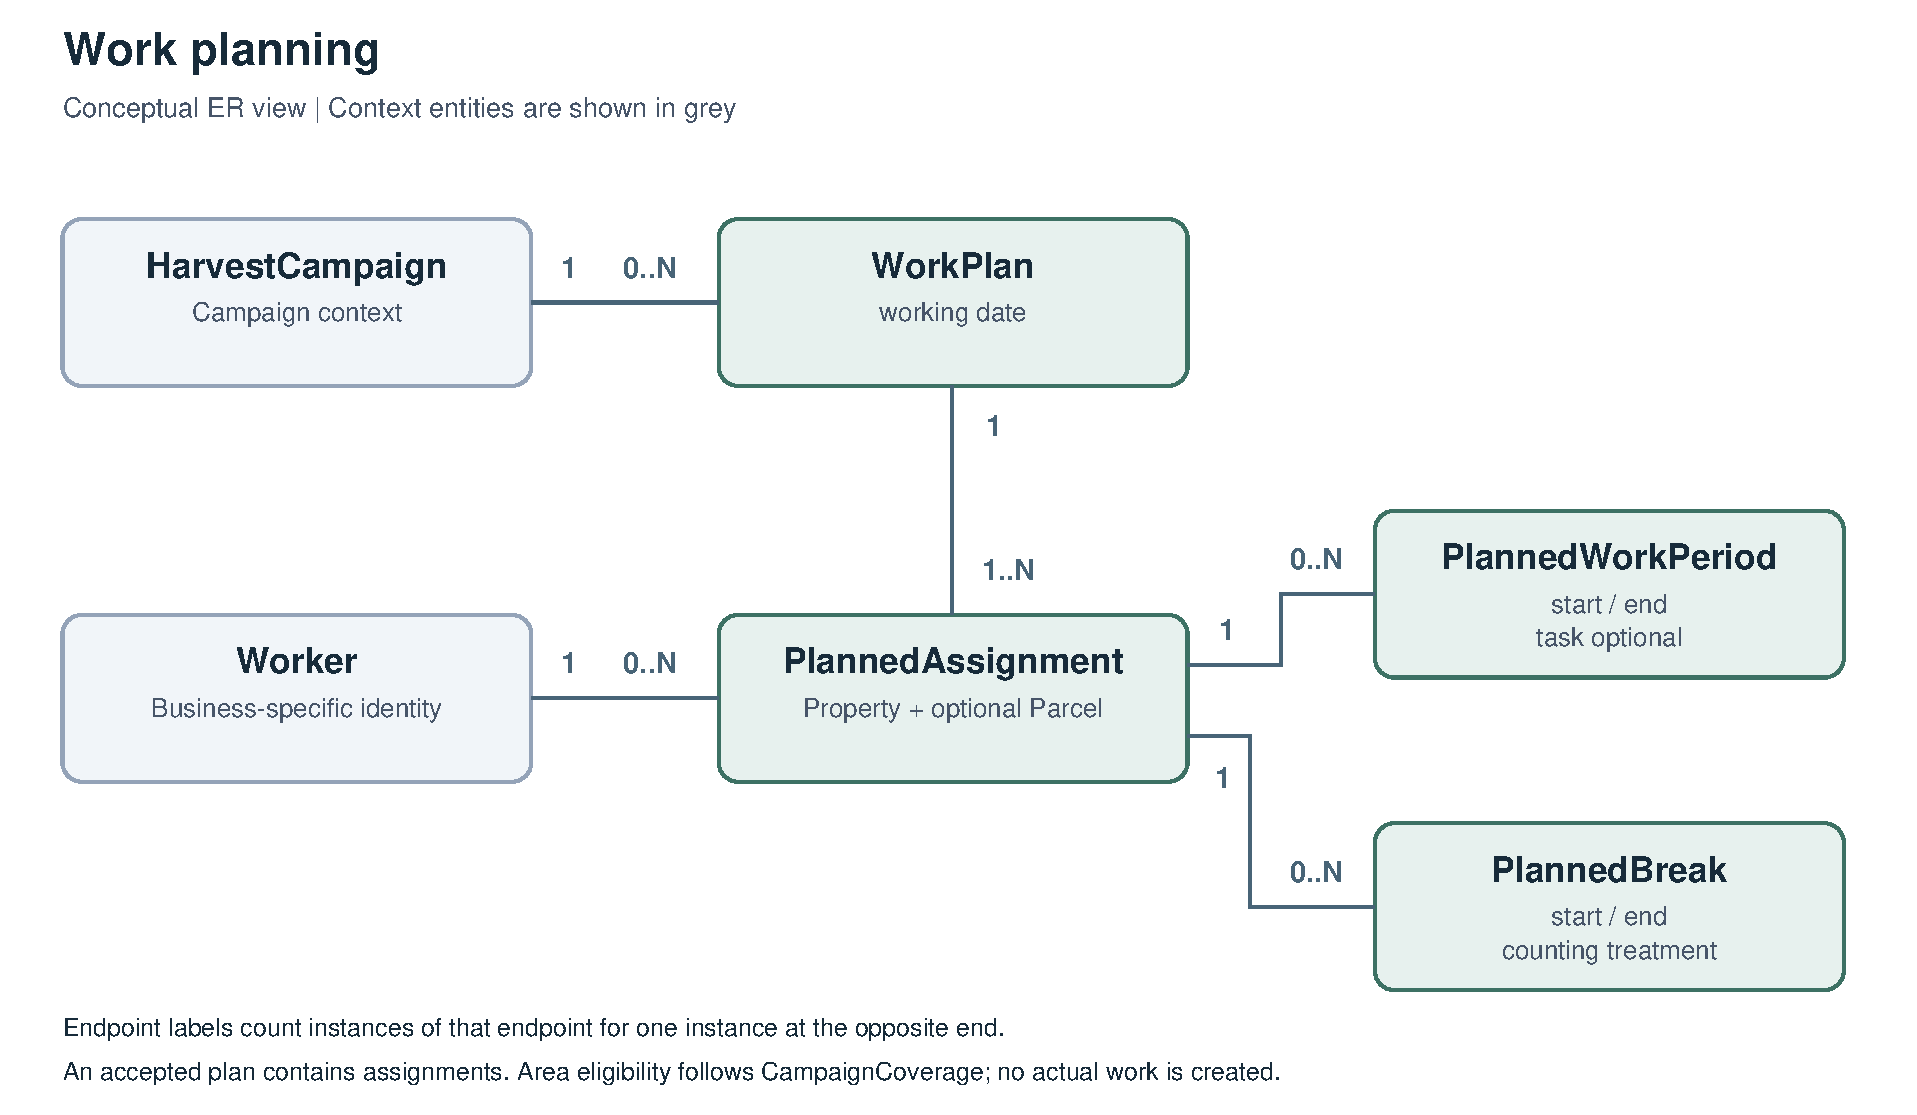
\includegraphics[width=\textwidth]{figures/er-planning.pdf}
    \caption{Conceptual relationships for work planning.
    Context entities are shown in grey; area references are summarised.}
    \label{fig:er-planning}
\end{figure}

\paragraph{Daily presence and campaign participation.}
DailyAttendance identifies one worker and working date within a workspace, without
a campaign reference. ActualWorkAssignment supplies the campaign and area context.
This supports one daily attendance decision across several campaigns and records
participation before hours or tasks are complete. An actual assignment may refer
to a source PlannedAssignment, but no mandatory one-to-one correspondence is imposed.

\begin{figure}[!htbp]
    \centering
    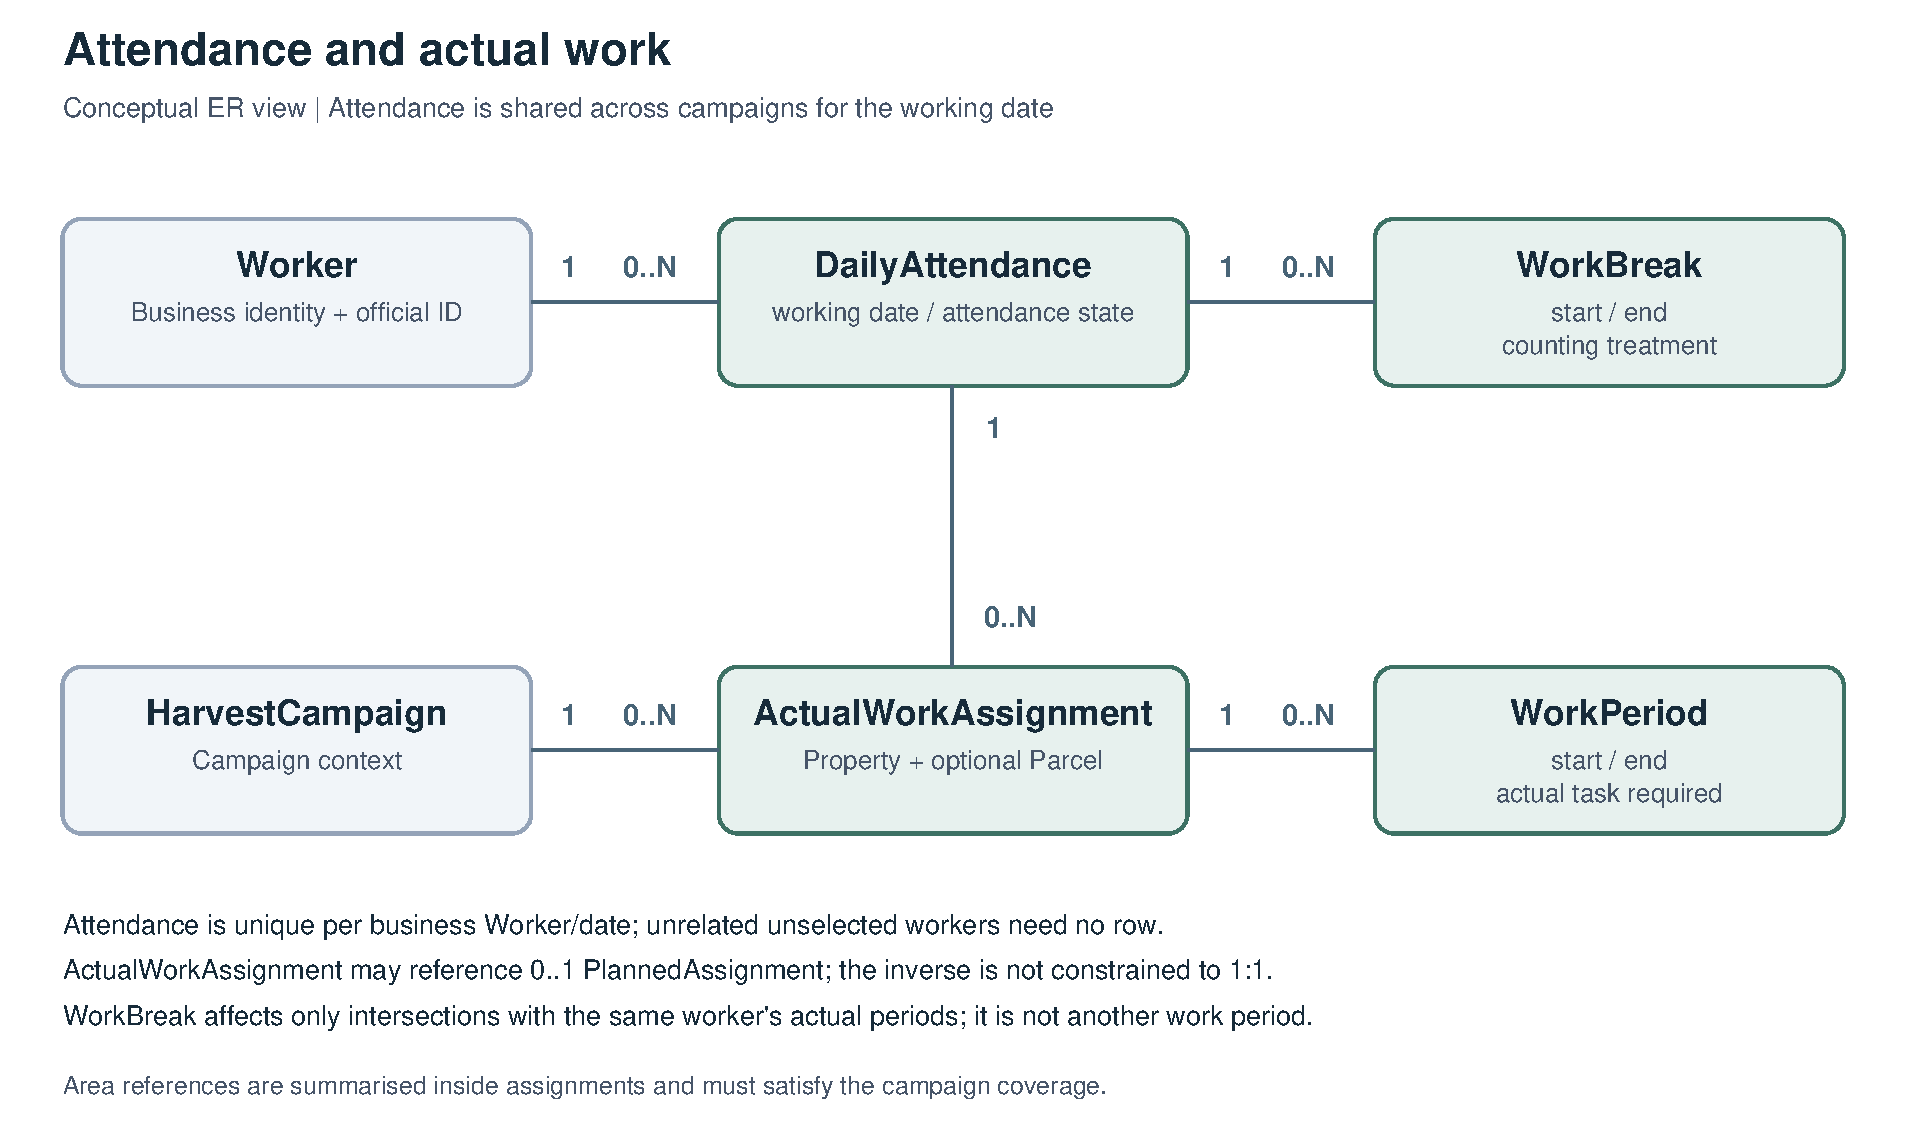
\includegraphics[width=\textwidth]{figures/er-actual-work.pdf}
    \caption{Conceptual relationships for daily attendance and actual work.
    The optional reference to a planned assignment does not impose a one-to-one correspondence.}
    \label{fig:er-actual-work}
\end{figure}

\paragraph{Intervals and breaks.}
WorkPeriod belongs to an actual assignment; WorkBreak belongs to daily attendance.
The latter placement lets a worker's break intersect consecutive task or campaign
periods without duplicating it. Complete start/end timestamps support intervals
crossing midnight and cross-campaign overlap checks. Missing hours are represented
by the absence of complete periods; each confirmed complete period requires
its actual task. An incomplete assignment is not converted into zero hours.

Planning and confirmation conditions are defined in \hyperref[br:017]{\identifier{BR-017}}--\hyperref[br:021]{\identifier{BR-021}};
the counted-time formula is in Section~\ref{sec:counted-working-time}.
Completion and correction use Sections~\ref{sec:completion-correction} and~\ref{sec:work-corrections}, without a separate
entity for every historical field value.

\paragraph{Expected versus unrelated workers.}
DailyAttendance is sparse: it does not require a row for every worker/date. Derive
expectations from selected/planned or actual assignments under
\hyperref[br:018]{\identifier{BR-018}}. This avoids recording non-selection as absence. Pending
records reference locally created Worker UUIDs without creating a second daily
attendance after acceptance.
